%
% File: chap02.tex
%
\let\textcircled=\pgftextcircled
\chapter{Results}
\label{chap:result}

\initial{T}his report shows that at an aimed 850 kW of thermal power, based on the NP1000 detector, the actual thermal power output measured is 910 kW. All three detectors in the reactor (NM1000, NPP1000 and NP1000) display a lower than measured thermal power output (respectively 840, 870 and 850 kW). This discrepancy can be caused by badly calibrated instruments. This section shows the results, based on the data available in the appendix~\ref{app:app02}, and discuss the associated uncertainties.

%=======
\section{Power calibration results}
\label{sec:powercalibres}

As can be seen in figure~\ref{fig:powercal} and table~\ref{tab:data}, the measured actual thermal ouput after 45 minutes is 910 kW. This value is 7\% higher than expected if the instruments were correctly calibrated. This is troublesome, since it would mean that the reactor reaches full power when the command control readings are around 930 kW, and that higher displayed power would be in excess of the licensed 1000 kW for the reactor operations. This would not have any impact on the reactor safety, but could be seen as a violation of the steady-state operational limits by the NRC.

One possible explanation, else than the apparent need for a adjustment of the instruments position or the uncertainties, would be the presence of 8 inches beam tube in the reactor during the power calibration. This could isolate part of the water in the tank and reduce the amount of water to which the heat is transferred. However, a quick calculation shows that this is unlikely to be (solely) responsible for the high difference observed between measured thermal power and readings from the three detectors.

Indeed, in order to compensate for the 7\% relative difference from the mass of water only, the real water level would need to be at around 22 inches below the upper lip of the tank. Considering the dimension of the tank, 7 ft 8 inches in diameter and 24 ft 9.25 inches in height, this represents around 575 gallons of water to be accounted for. The 8 inches beam tube, assuming a conservative 8 inches diameter and a 24 ft 9.25 inches height, would only account for 65 gallons, moreover not completely insulated, the aluminium clad being quite conductive. The mass and heat capacity of this cladding would also not have a consequent impact on the system's heat constant.

\begin{figure}[t!]
	\centering
	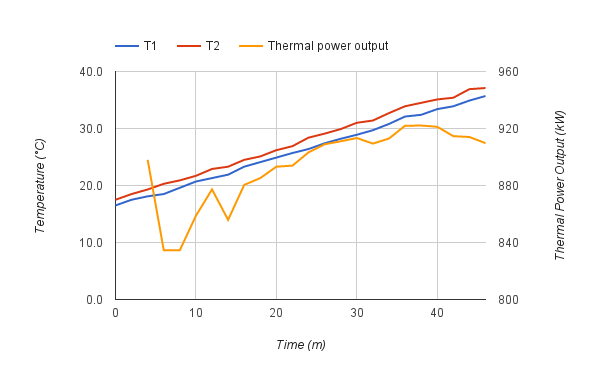
\includegraphics[height=0.4\textheight]{fig02/calibration}
	\mycaption[Power calibration of the GSTR]{Power calibration of the GSTR.}
	\label{fig:powercal}
\end{figure}

One thing that can be noted is the fact that the graph is not extremely stabilized yet after 46 minutes. In the figure~~\ref{fig:powercal}, the first aberrant point was taken off while still considered in the slope calculation. A real suppression of this point gives the same thermal power output, 910 kW.


\section{Uncertainties}
\label{sec:uncertainties}

The two sensors used presents some uncertainties in their measurements. $T_1$ sensor, the temporary water temperature instrument is a 2252 ohm Resistance Temperature Device detector, with an accuracy of $\pm0.3$\% + 0.3\degree C and a repeatability of 0.1\degree C. The permanently installed water temperature instrument, $T_2$, is a 100 ohm RTD presenting an accuracy of $\pm0.2$\degree C, and a $\pm1$\% linearity.

A quick calculation of the minimum and maximum measured thermal power output was done, by taking into account the probes uncertainties. It is important to note that given the asymmetric uncertainties given for the temporary probe, and the mix of percentage and absolute errors, this simple computation is likely false. Nonetheless, it can give an idea of the uncertainties we are dealing with.

The principle of this method is to consider the uncertainty ranges of temperatures measured at each time step, and to compute the smallest and biggest slopes based on these ranges. This gives us a rough minimum and maximum value for the measured thermal power output.


\begin{equation}\label{eq5}
\begin{aligned}
S_{min, (i,j)} = \frac{y_{min, (i,j)} - y_{max, (i,0)}}{x_{i,j} - x_{i,0}} \\
S_{max, (i,j)} = \frac{y_{max, (i,j)} - y_{min, (i,0)}}{x_{i,j} - x_{i,0}}
\end{aligned}
\end{equation}

\begin{equation}\label{eq6}
\begin{aligned}
P_{min, kW} = \frac{\sum\limits_{i=1}^{N}{\frac{1000*60*S_{min, (i,j)}}{H}}}{N} \\
P_{max, kW} = \frac{\sum\limits_{i=1}^{N}{\frac{1000*60*S_{max, (i,j)}}{H}}}{N}
\end{aligned}
\end{equation}

The detailed results are presented in tables~\ref{tab:data_t1},~\ref{tab:data_t2} and~\ref{tab:data_power}. It can be seen that the minimal thermal power output obtained when considering the most disadvantageous combinations of probes uncertainties is 854 KW, while the maximum is 928 kW. This shows a wide range of error, which can potentially explain the high value obtained during the power calibration, if both the probes were performing at the highest and lowest end of their respective range.
